%%%%%%%%%%%%%%%%%%%%%%%%%%%%%%%%%%%%%%%%%
% Simple Sectioned Essay Template
% LaTeX Template
%
% This template has been downloaded from:
% http://www.latextemplates.com
%
% Note:
% The \lipsum[#] commands throughout this template generate dummy text
% to fill the template out. These commands should all be removed when 
% writing essay content.
%
%%%%%%%%%%%%%%%%%%%%%%%%%%%%%%%%%%%%%%%%%

%----------------------------------------------------------------------------------------
%	PACKAGES AND OTHER DOCUMENT CONFIGURATIONS
%----------------------------------------------------------------------------------------

\documentclass[12pt]{article} % Default font size is 12pt, it can be changed here
\usepackage{geometry} % Required to change the page size to A4
\geometry{a4paper} % Set the page size to be A4 as opposed to the default US Letter

\usepackage{graphicx} % Required for including pictures
\usepackage{float} % Allows putting an [H] in \begin{figure} to specify the exact location of the figure


\usepackage[T1]{fontenc} %codage
\usepackage[english,francais]{babel}
\usepackage[utf8]{inputenc} %codage
\usepackage{lmodern}
\usepackage{amssymb}
\usepackage{amsmath}

\usepackage{amsthm}

\usepackage{url}

\usepackage{tikz}         
\usetikzlibrary{mindmap}

\linespread{1.2} % Line spacing

%\setlength\parindent{0pt} % Uncomment to remove all indentation from paragraphs





\begin{document}

%----------------------------------------------------------------------------------------
%	RE-DEFINITION 
%----------------------------------------------------------------------------------------
% MATHS
%-----------

\newtheorem{Definition}{Definition}
\newtheorem{Theorem}{Theorem}
\newtheorem{Proposition}{Proposition}
\newtheorem{Corollary}{Corollary}
\newtheorem{Problem}{Problem}
\newtheorem{Lemma}{Lemma}
 
\newcommand{\RefSec}[1]{Section~\ref{#1}}
\newcommand{\RefFig}[1]{Fig.~\ref{#1}}
\newcommand{\RefTab}[1]{Tab.~\ref{#1}}
\newcommand{\RefDef}[1]{Definition~\ref{#1}}
\newcommand{\RefPro}[1]{Proposition~\ref{#1}}
\newcommand{\RefLem}[1]{Lemma~\ref{#1}}
\newcommand{\RefThe}[1]{Theorem~\ref{#1}}
\newcommand{\Eq}[1]{(\ref{#1})}

% LINES
%-----------
\newcommand{\HRule}{\rule{\linewidth}{0.5mm}} % Defines a new command for the horizontal lines, change thickness here

%----------------------------------------------------------------------------------------
%	TITLE PAGE
%----------------------------------------------------------------------------------------

\begin{titlepage}

\center % Center everything on the page

\textsc{\LARGE Laboratoire d'InfoRmatique en Image et Syst\`{e}mes d'information}\\[1.5cm] % Name of your university/college
%\textsc{\Large }\\[0.5cm] % Major heading such as course name
\textsc{\large Rapport de stage}\\[0.5cm] % Minor heading such as course title

\HRule \\[0.4cm]
{ \huge \bfseries Structure du bord des disques discrets}\\[0.4cm] % Title of your document
\HRule \\[1.5cm]

\begin{minipage}{0.4\textwidth}
\begin{flushleft} \large
\emph{Auteur:}\\
Thomas \textsc{Lafond} % Your name
\end{flushleft}
\end{minipage}
~
\begin{minipage}{0.4\textwidth}
\begin{flushright} \large
\emph{Encadrant:} \\
Tristan \textsc{Roussillon} % Supervisor's Name
\end{flushright}
\end{minipage}\\[4cm]

{\large 3 Juillet 2013}\\[3cm] % Date, change the \today to a set date if you want to be precise

%\includegraphics{Logo}\\[1cm] % Include a department/university logo - this will require the graphicx package

\vfill % Fill the rest of the page with whitespace

\end{titlepage}

%----------------------------------------------------------------------------------------
%	TABLE OF CONTENTS
%----------------------------------------------------------------------------------------

\tableofcontents % Include a table of contents

\newpage % Begins the essay on a new page instead of on the same page as the table of contents 

%------------------------------------------------
\section{Introduction}
%------------------------------------------------

%-----------------------------------------------------------------
\subsection{Contexte pédagogique}
%-----------------------------------------------------------------

% Parcours - ok
Actuellement en deuxième année du master professionnel de Mathématiques : Statistiques, Informatique et Techniques Numériques (SITN) à l’Université Claude Bernard - Lyon 1, je me dois de réaliser un stage dans le but de valider ma formation et d'ainsi obtenir mon diplôme. \newline

%labo -ok
Je suis actuellement accueilli pour une durée de 6 mois au LIRIS - Laboratoire d'InfoRmatique en Image et Systèmes d'information - UMR 5205 CNRS. Le LIRIS est issue de la fusion de plusieurs pôles de recherche de la région Lyonnaise. Aujourd'hui composé d'environ 300 personnes, il participe activement à la recherche et à l'éducation à travers ses deux grands départements thématiques : "Image" et "Données, Connaissances, Services".\newline

%encadrant
Je suis encadré par Tristan Roussillon, Maitre de conférence à l'Insa - Institut National des Sciences Appliquées et membre de l'équipe M2Disco - Modèles Multirésolution, Discrets et Combinatoires. Cette équipe est une composante du département Image du LIRIS qui traite de sujet comme l'analyse d'images, l'optimisation, la programmation par contraintes et la géométrie discrète. C'est d'ailleurs sur cette dernière branche que le contexte de mon stage c'est déroulé.



%-----------------------------------------------------------------
\subsection{Contexte scientifique}
%-----------------------------------------------------------------

J'ai découvert pour l’occasion la géométrie discrète, se nommant également sous le nom plus générique de digital geometry dans la langue de Shakespeare. Cette discipline de recherche gravite à l'intersection de bien des domaines mathématiques et informatiques.\\

(pics)\\

Il s'agit principalement d'étudier la géométrie et la topologie d'objets portés par des structures régulières. Nous intéressons plus particulièrement au disque discret sur la grille $\mathbb{Z}^{2}$. 


%------------------------------------------------
\section{Motivations}
%------------------------------------------------

%-----------------------------------------------------------------
\subsection{Le bord du disque discret}
%-----------------------------------------------------------------

%-----------------------------------------------------------------
\subsubsection{Du disque Euclidien au disque discret}


Le disque discret $\mathcal{D}$ est défini par analogie avec le disque Euclidien $\mathcal{D}_e$ qui représente l'ensemble des points situé à une distance inférieur à $R$ de son centre $O$.


\begin{Definition}{Disque fermé Euclidien}
\label{def:disk-euc}
 $$\mathcal{D}_e =  \left\{ p=(x,y) \in \mathbb{R}^{2} |  (x - u)^2 + (y - v)^2 \leq R^2 \right\}$$
\end{Definition}

\begin{Definition}{Disque fermé discret}
\label{def:disk-dis}
  $$\mathcal{D} =  \left\{ p=(x,y) \in \mathbb{Z}^{2} |  ax + by + c( x^2 + y^2 ) + d = 0. \right\}$$
  
  avec $(u,v) = ( -a/(2c) , -b/(2c) )) \in \mathbb{Z}^{2}$ les coordonnées du centre et $R = \sqrt{ (a^2 + b^2 - 4cd) / 4c^2 } \in \mathbb{Z}^{+*}$ le rayon.\\
\end{Definition}

\begin{figure}[H]
  \centering
  \includegraphics[width=6cm]{fig/2-mot/circle/circle-euc-0.pdf}
  \includegraphics[width=6cm]{fig/2-mot/circle/circle-dis-0.pdf}
  \caption{Disque Euclidiens et Discret}
\end{figure}


Si la définition du disque fermé discret dans $\mathbb{Z}^{2}$ (appelé pour la suite du rapport uniquement disque discret) reste très proche de la définition Euclidienne, l'équivalent discret de son cercle afin de récupérer tous les points du bord change quant à elle considérablement. L'ensemble des points représentés en rouge sur le dessin, appartenant à l'ensemble : $\left\{ (x,y) \in \mathbb{Z}^{2} |  (x - u)^2 + (y - v)^2 = R^2 \right\}$, étant donc positionnés exactement sur le cercle Euclidien ne suffisent pas pour représenter le disque discret et son ensemble de points sur le bord. Il faut choisir une définition plus générale.

\begin{Definition}{Cercle Euclidien}
\label{def:cer-euc}
  $$\mathcal{C}_e =  \left\{ (x,y) \in \mathbb{R}^{2} |  (x - u)^2 + (y - v)^2 = R^2 \right\}$$
  avec $(u,v) \in \mathbb{R}^{2}$ les coordonnées du centre et $R \in \mathbb{R}^{+*}$ le rayon.\\
\end{Definition}

\begin{Definition}{Cercle discret}
\label{def:cer-dis}
  $$ \mathcal{C} =  \left\{ p=(x,y) \in \mathbb{D} | \exists q \notin \mathbb{D} | d(p, q) = 1  \right\}$$
\end{Definition}

\begin{figure}[H]
  \centering
  \includegraphics[width=6cm]{fig/2-mot/circle/circle-dis-1.pdf}
  \caption{Cercle Euclidiens}
\end{figure}
%PICS et PICS de disque et de cercle euclidien


%-----------------------------------------------------------------
\subsubsection{L'étude des points du bord}

À partir de la définition précédente du cercle discret, il est possible de formuler plusieurs remarques. De par le fait de travailler sur $\mathbb{Z}^{2}$, on sait que les points sont ordonnées sur une grille régulière. Pour chaque point, il est possible d'atteindre quatre voisins en se dirigeant d'une unité vers les quatre points cardinaux. Chaque point possède donc un voisin, en haut, à gauche, en bas et à droite de lui. Or, on observe que les points strictement à l'intérieur du disque discret et non sur le bord (en bleu clair) possèdent tous leurs quatre voisins à l'intérieur du disque (maillage en rouge).

\begin{Definition}{Ensemble de points strictement à l'intérieur d'un disque}
\label{def:cer-dis}
  $$ \stackrel{\ \circ}{D} =  \left\{ p=(x,y) \in \stackrel{\ \circ}{D} | d(p, q) = 1 \Rightarrow q \in \mathcal{D} \right\}$$
\end{Definition}

Pour autant, les points du bords du disque discret \RefDef{def:cer-dis}, possèdent eux une distribution différente. Chacun des points du bord possède entre un et trois voisins à l'extérieur du disque (en vert clair).

\begin{figure}[H]
  \centering
  \includegraphics[width=6cm]{fig/2-mot/circle/circle-dis-2.pdf}
  \includegraphics[width=6cm]{fig/2-mot/circle/circle-dis-3.pdf}
  \caption{Voisins des points strictement à l'intérieur et sur le bord }
\end{figure}

On se retrouve alors avec deux ensembles disjoints pour définir et représenter un disque discret. Le premier est bien ordonnée. Il représente les points strictement à l'intérieur du disque. Le deuxième ensemble représente les points du bord du disque et propose une distribution de points non régulière. De part la régulartité du premier, seule l'étude des points du bord nous semble pertinente pour comprendre l'organisation et la structure des disque discret.


%-----------------------------------------------------------------
\subsection{Alpha-Shape}
%-----------------------------------------------------------------

%-----------------------------------------------------------------
\subsubsection{Définition générale}

En s'intéressant principalement à des contours de formes discrètes, un ensemble d'outil nous est apparu comme particulièrement opportun. Il s'agit des $\alpha$-hull et des $\alpha$-shape définit pour la première fois dans \cite{EdeKirSei83} de la manière suivante.\\



\begin{Definition}{$\alpha$-hull de $\mathcal{S}$}
\label{def:ah-txt}
    Intersection de tous les disques généralisés de rayon $1/\alpha$ qui contiennent tous les points de l'ensemble.
\end{Definition}

Un disque généralisé permet de définir des disques avec des rayons négatifs en faisant appel au complémentaire.

\begin{Definition}{Disques génralisés de rayon $1/\alpha$}
\label{def:ah-txt}
   Si $\alpha > 0$, $\mathcal{D}_{\alpha}$ est le disque fermé de rayon $1/\alpha$.\\
   Si $\alpha > 0$, $\mathcal{D}_{\alpha}$ est le complémentaire fermé du disque de rayon $1/\alpha$.
\end{Definition}

On en déduit une nouvelle définition pour les $\alpha$-hulls.

\begin{Definition}{$\alpha$-hull de $\mathcal{S}$}
\label{def:ah}
    $$\left\{ \cap \mathcal{D}_{\alpha} | \forall (x,y)\in \mathcal{S} \Rightarrow (x,y) \in \mathcal{D}_{\alpha} \right\}$$
\end{Definition}

\begin{figure}[h!]
  \centering
  \includegraphics[width=0.4\linewidth,page=1]{fig/2-mot/as/mot-alpha-shape.pdf}
  \includegraphics[width=0.4\linewidth,page=3]{fig/2-mot/as/mot-alpha-shape.pdf}
  \caption{$\alpha$-Hull négative et $\alpha$-Hull positive }
\end{figure}

       

Les sommets de $\alpha$-hull sont appelés points $\alpha$-extreme. S'ils sont relié par un arc de cercle de rayon 1/ $\lvert \alpha \rvert$ qui n'exclue pas de points, on dit alors qu'ils sont adjacents.

\begin{Definition}{$\alpha$-shape}\\
\label{def:as}
      Graphe "plongé" reliant tous les $\alpha$-extremes adjacents par des segments de droite discrète.
\end{Definition}

\begin{figure}[h!]
  \centering
  \includegraphics[width=0.4\linewidth,page=2]{fig/2-mot/as/mot-alpha-shape.pdf}
  \includegraphics[width=0.4\linewidth,page=4]{fig/2-mot/as/mot-alpha-shape.pdf}
  \caption{$\alpha$-Shape négative et $\alpha$-Shape positive }
\end{figure}

L'utilité des $\alpha$-shapes est d'être une sous-ensemble des points du bord. 
% need more

%-----------------------------------------------------------------
\subsubsection{$\alpha$-shapes de disque discret}

En prenant un panel assez large d'$\alpha$-shape avec $\alpha$ succéssivement négatif et positif variant de -2 à $R_D$ (le rayon du disque) on remarque que les $\alpha$-shapes représentent un large panel d'ensemble représentatif des points du bord d'un disque discret.

%PICS avec alpha shapes de disque.

%-----------------------------------------------------------------
\subsubsection{Plusieurs remarques}

\paragraph{}
Le cas central de $\alpha = 0$ représente une intersection de disque de rayon infini, cela peut être interprété comme une intersection de demi-plan. On retrouve exactement l'enveloppe convexe.

\paragraph{}
Les plus petits $\alpha = -2$ et $\alpha = -\sqrt{2}$ représenter les bords. En effet, en ne pouvant s'éloigner au plus de disques de rayon $1/2$ et $\sqrt{2}/2$, on ne peut suivre le bord de nos disques que par l'intermédiaire des voisins 4-connexes et 8-connexes de chaque point du bord.

\paragraph{}
En réalisant l'union de nos $\alpha$-shape pour le cas négatif et le cas positif, on s'appuie également sur les triangulations d'ordre 0 et n de Delaunay. 
% need more 


%------------------------------------------------
\section{Méthodes de calculs existantes}
%------------------------------------------------

%-----------------------------------------------------------------
\subsection{Suivi de Bord}
%-----------------------------------------------------------------

La méthode du suivi du bord d'un disque discret est un processus étudié et connu. Elle est sensiblement la même suivant le cas souhaité : 4-connexes ou 8-connexes. Elle se décompose en deux étapes. Trouver un point sur le bord, puis chercher le point suivant de manière répétée jusqu'à retrouver le premier point et refermer le bord.

%-----------------------------------------------------------------
%\subsubsection{Trouver le sommet de départ}

Pour chercher un point de départ sur le bord du disque discret à partir de la seule connaissance de ses paramètres, nous avons choisi de récupérer le point d'ordonnée minimale et d'abscisse maximale à l'intérieur du disque. Nous prenons le point de $\mathbb{Z}^2$ avec les coordonnées entières du centre du disque. Puis, nous descendons le long de l'axe vertical d'une longueur entière égale au rayon pour trouver un point d'ordonnée minimale. Ensuite, nous translatons suivant l'axe horizontal afin de récupérer le point d'abscisse maximal. (Illustré \textsc{figure} \ref{fig:depart}.) On note \textbf{a} ce point de départ. Cette procédure prend un temps constant. 

\begin{figure}[H]
  \centering
  \includegraphics[width=0.3\linewidth,page=1]{fig/4-exi/suivi/exi-depart-0.pdf}
  \includegraphics[width=0.3\linewidth,page=1]{fig/4-exi/suivi/exi-depart-1.pdf}
  \caption{Recherche du premire point $a$ à partir du centre et du rayon du disque.}
\label{fig:depart}
\end{figure}
  

%-----------------------------------------------------------------
%\subsubsection{Trouver le sommet suivant}

La deuxième étape consiste à trouver le sommet suivant appartenant au bord. On répète cette étape jusqu'à retrouver le point a.

A partir d'un point quelconque du bord $p$ ($a$ au début), le point suivant est choisi suivant la position des 4 voisins (resp 8 voisins) de $p$ par rapport au disque et d'un sens arbitraire de rotation. En tournant dans le sens trigonométrique et en partant d'un voisin situé à l'extérieur du disque, le point suivant est le premier voisin situé à l'intérieur du disque. 

\begin{figure}[H]
  \centering
  \includegraphics[width=0.4\linewidth,page=1]{fig/4-exi/suivi/exi-suivi-0.pdf}
  \caption{Suivi de bord 4-connexes et 8-connexes}
\end{figure}
  
Cette étape prend un temps constant, limité par la taille constante du voisinage. Elle est répétée autant de fois qu'il y a de points sur le bord du disque. Rappelons que $R$ est le rayon du disque. Comme il y a $O(R)$ points sur le bord du disque, la complexité en temps du suivi est en $O(R)$. 

%-----------------------------------------------------------------
\subsection{Enveloppe Convexe : Algorithme de Har-Peled}
%-----------------------------------------------------------------

De nombreux algorithmes existent pour calculer l'enveloppe convexe d'un ensemble de points. L'algorithme de Graham \cite{Graham1972} l'implémente en $O(n \log n)$ pour un ensemble quelconque de $n$ points. Quand les $n$ points sont ordonnés, comme le sont les points du bord d'un disque discret, le parcours de Graham est en $O(n)$. Par conséquent, calculer l'enveloppe convexe des points d'un disque discret se calcule par suivi de bord et parcours de Graham en $O(R)$. Cependant un algorithme géométrique introduit par Har-Peled en 1998 \cite{HarPeled98} calcule l'enveloppe convexe des points d'un disque discret de manière incrémentale et ``output-sensitive''.
%% reference pour Graham
%% reference pour Har-Peled

\begin{Definition}{Output sensitive}\\
\label{def:os}
      Un algorithme output sensitive possède un temps d’exécution qui dépend de la taille de sa sortie.
\end{Definition}

La méthode de Har-Peled dépend du nombre de sommets de l'enveloppe convexe. Elle construit successivement les arêtes du polygone à l'aide des convergents qui représente le pendant géométrique du calcul du pgcd de deux nombres entiers (voir l'annexe \ref{annexe-euc-geo}). La complexité en temps de cet algorithme pour un disque de rayon $R$ relève d'une part de la recherche du prochain sommet en $O(\log R)$ et également du nombre de sommets qui est $O(R^{2/3})$. Soit une complexité totale en temps de $O( R^{2/3} \log R)$.

%-----------------------------------------------------------------
\subsubsection{Calcul des convergents}

Cette méthode de calcul est géométrique. Soient l’origine $O=(0,0)$ et $P = (P_x, P_y)$ un point à coordonnées entières. Nous cherchons le premier point de $\mathbb{Z}^{2}$ appartenant au segment de droite [O,P]. Le coefficient trouvé correspond au pgcd de $P_x$ et $P_y$.\\

Soient $p_{-2} = (1,0)$ et $p_{-1} = (0,1)$ les deux premiers convergents. Pour trouver les convergents suivants, nous mettons en place une méthode récursive :

$$p_{k} = p_{k-2} + q_k p_{k-1}$$

où $q_k$ est le plus grand entier tel que $p_{k}$ et $p_{k-2}$ soient du même côté de la droite.\\

L'opération correspond à jeter un rayon de $p_{k-2}$ dans la direction de $p_{k-1}$ pour étudier l’intersection du vecteur et du segment de droite de direction $y_P / x_P$. La méthode s’arrête quand un convergent $p_{k}$ est exactement sur la droite.\\

\begin{figure}[H]
  \centering
  \includegraphics[width=0.4\linewidth]{fig/4-exi/har/exi-har-0.pdf}
  \includegraphics[width=0.4\linewidth]{fig/4-exi/har/exi-har-1.pdf}
  \caption{Calcul des convergents du point (3,8)}
  \label{fig:conv}
\end{figure}

Le calcul des convergents est illustré en \textsc{figure} \ref{fig:conv} avec le point (3,8). Après avoir positionné $p_{-2} = (1,0)$ et de $p_{-1} = (0,1)$, on calcule successivement $p_{0} = p_{-1} + 2p_{-2} = (1,2)$,  $p_{1} = p_{-1} + p_{0} = (1,3)$. On obtient $p_{2} = p_{0} + 2p_{1} = (3,8)$, le premier point sur le segment. 3 et 8 sont premiers entre eux.

%-----------------------------------------------------------------
\subsubsection{Passage au disque}


La méthode de calcul de l'enveloppe convexe d'un disque se décompose en deux étapes. La première consiste à trouver un point de départ. Nous appliquons la même procédure que lors du suivi de bord pour récupérer le point de départ d'ordonnée minimale et d'abscisse maximale. Par définition ce point appartient à l'enveloppe convexe.\\

Ensuite, nous cherchons le sommet suivant jusqu'à retrouver le point de départ. Cette étape est réalisée en calculant les convergents les plus proches du bord du disque. Nous allons alternativement être à l'intérieur du disque lorsque $k$ est impair et à l'extérieur du disque lorsque $k$ est pair. Nous repartons d'un convergent s'il se situe exactement sur le bord du disque. Sinon, nous repartons du dernier convergent de degré impair lorsque que le lancer de rayon n'intersecte pas notre disque.\\
%% effectif: pas clair 
%% liens avec la figure ?

\begin{figure}[H]
  \centering
  \includegraphics[width=0.4\linewidth]{fig/4-exi/har/exi-har-10.pdf}
  \includegraphics[width=0.4\linewidth]{fig/4-exi/har/exi-har-11.pdf}
  \caption{Calcul de l'enveloppe convexe d'un disque}
\label{fig:disque-conv}  
\end{figure}

L'application de l'algorithme pour s'illustré en \textsc{figure} \ref{fig:disque-conv} en partant d'un sommet sur l'origine. Avec $p_{-2} = (1,0)$ et de $p_{-1} = (0,1)$, on trouve $p_{0} = p_{-1} + 2p_{-2} = (1,2)$ à l'extérieur du cercle puis $p_{1} = p_{-1} + 2p_{0} = (2,5)$ à l'intérieur du cercle. Le rayon $p_{2}$ n'intersectant pas le disque, on arrête l'algorithme et on repart du dernier convergent à l'intérieur du disque : $p_{1}$.

\subsubsection{Résultats}

Les résultats illustrés \textsc{figure} \ref{fig:ch} et écrits \textsc{table} \ref{tab:ch} ont été obtenus en calculant sur une moyenne de 100 disques de rayon $2^k$ possédant un centre à coordonnée rationnel compris dans $[0,1]\times[0,1]$. Afin de vérifier la convergence en $O(R^{2/3})$, nous avons également récupéré la moyenne par rayon de la division du nombre de sommets de l'enveloppe convexe sur le rayon à la puissance 2/3. La zone bleue de la figure correspond à l'intervale entre le minimum et le maximum obtenu.

On s'intéresse également à vérifié la complexité en temps de notre algorithme. On le compare à la marche de Graham sur la \textsc{figure} \ref{tab:ch-time}. 

\begin{figure}[H]
  \centering
  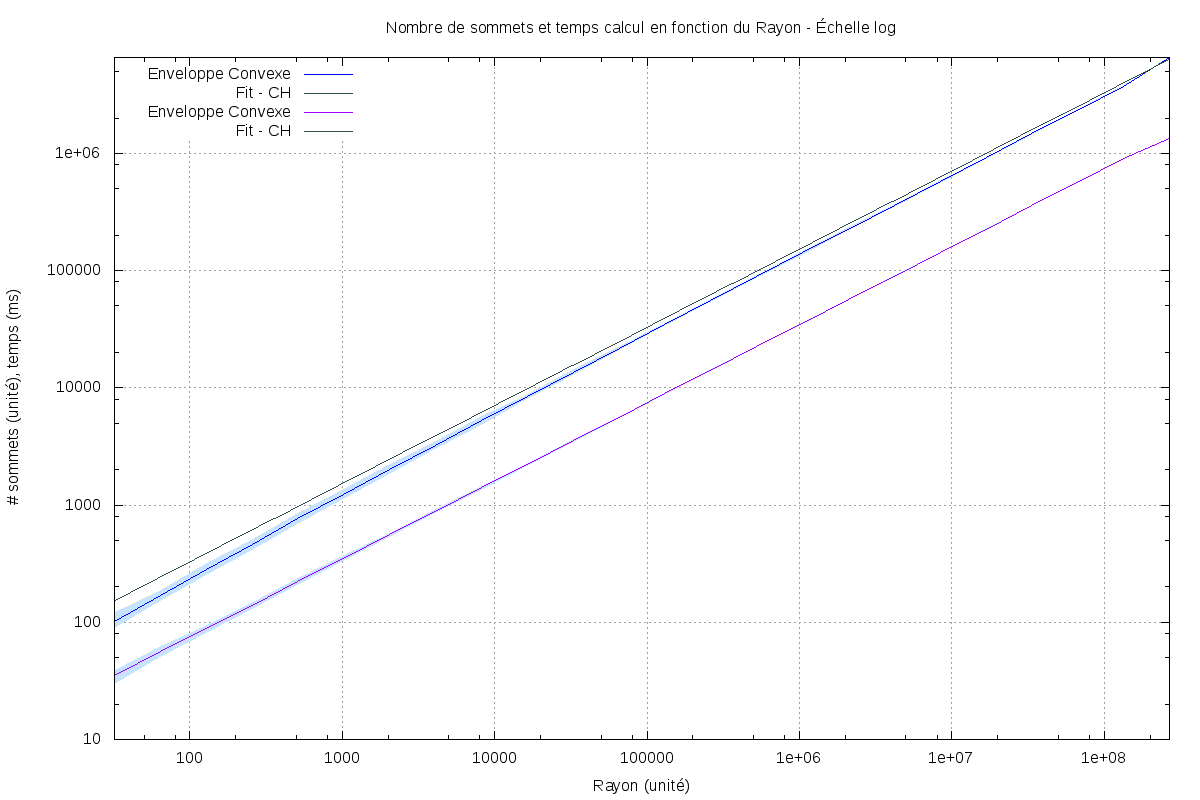
\includegraphics[width=\linewidth]{fig/4-exi/ch/exi-ch-sommet.png}
  \caption{Sommets et bord de l'enveloppe convexe}
  \label{fig:ch} 
\end{figure}

\begin{table}[H]
  \begin{tabular}{|p{0.09\linewidth}|p{0.13\linewidth}||p{0.2\linewidth}|p{0.13\linewidth}||p{0.2\linewidth}|p{0.13\linewidth}|}
    \hline
    \multicolumn{2}{|c||}{Rayon} & \multicolumn{4}{c|}{Enveloppe convexe} \\  \hline 
    $R=2^k$  &  & \multicolumn{2}{c||}{Nombre de Sommets} &  \multicolumn{2}{c|}{Nombre de points sur le bord} \\ \hline 
    k & R &   & $\# / R^{2/3}$  &   & $\# / R^{2/3}$ \\    
    \hline
    5 & 32         & 35,36     & 3,51 & 102,05   &  10,12\\
    6 & 64         & 55,78     & 3,49 & 170,16   &  10,64\\
    7 & 128        & 87,78     & 3,46 & 283,69   &  11,17\\
    8 & 256        & 139,71    & 3,47 & 465,06   &  11,53\\
    9 & 512        & 222,07    & 3,47 & 761,01   &  11,89\\
    10 & 1024      & 351,72    & 3,46 & 1,24E+03 &  12,21\\
    11 & 2048      & 558,18    & 3,46 & 2,01E+03 &  12,45\\
    12 & 4096      & 883,86    & 3,45 & 3,24E+03 &  12,68\\
    13 & 8192      & 1,40E+003 & 3,45 & 5,25E+03 &  12,92\\
    14 & 16384     & 2,23E+003 & 3,45 & 8,41E+03 &  13,03\\
    15 & 32768     & 3,54E+003 & 3,45 & 1,35E+04 &  13,19\\
    16 & 65536     & 5,62E+003 & 3,46 & 2,16E+04 &  13,28\\
    17 & 131072    & 8,91E+003 & 3,45 & 3,47E+04 &  13,45\\
    18 & 262144    & 1,41E+004 & 3,45 & 5,54E+04 &  13,53\\
    19 & 524288    & 2,25E+004 & 3,45 & 8,87E+04 &  13,64\\
    20 & 1048576   & 3,56E+004 & 3,45 & 1,42E+05 &  13,75\\
    21 & 2097152   & 5,66E+004 & 3,45 & 2,26E+05 &  13,81\\
    22 & 4194304   & 8,98E+004 & 3,45 & 3,61E+05 &  13,88\\
    23 & 8388608   & 1,43E+005 & 3,45 & 5,76E+05 &  13,94\\
    24 & 16777216  & 2,26E+005 & 3,45 & 9,19E+05 &  14,02\\
    25 & 33554432  & 3,59E+005 & 3,45 & 1,46E+06 &  14,07\\
    26 & 67108864  & 5,70E+005 & 3,45 & 2,33E+06 &  14,10\\
    27 & 134217728 & 8,98E+005 & 3,42 & 3,74E+06 &  14,27\\
    28 & 268435456 & 1,35E+06  & 3,24 & 6,62E+06 &  15,90\\
    \hline
  \end{tabular} 
  \caption{Sommet et bord de l'enveloppe convexe}
  \label{tab:ch} 
\end{table}

\begin{figure}[H]
  \centering
  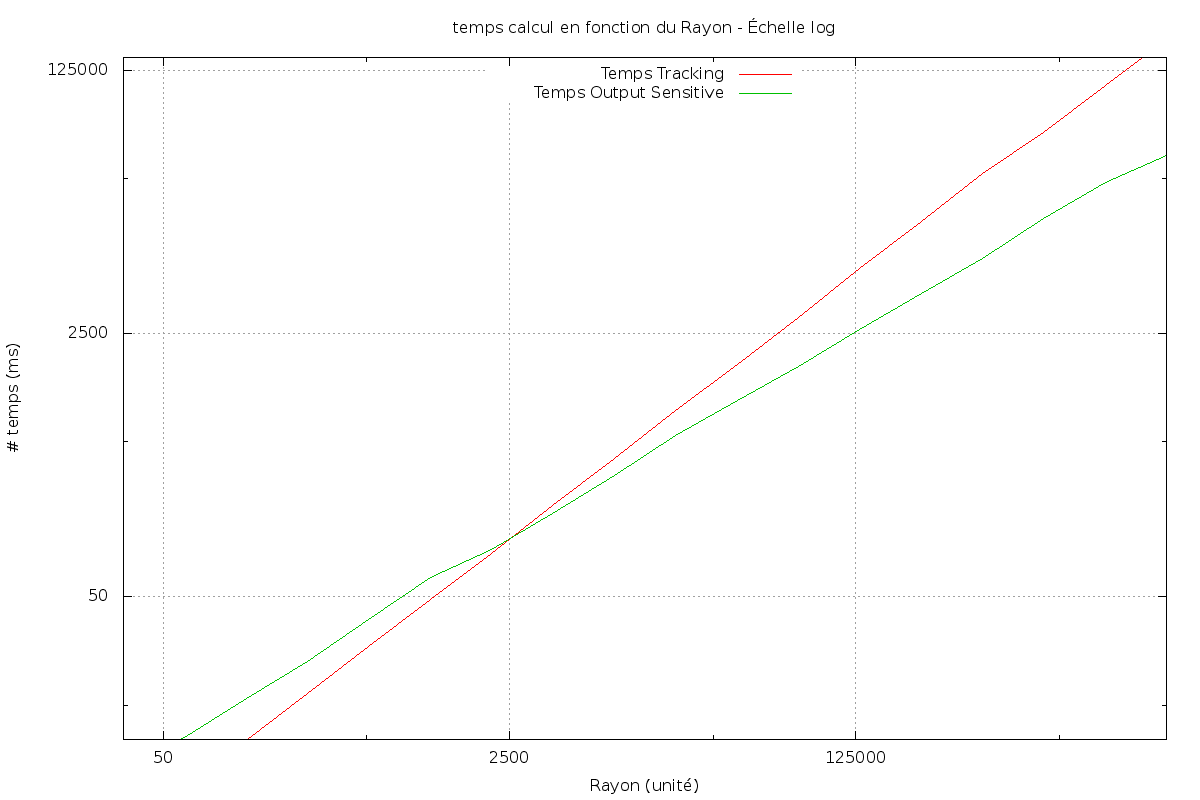
\includegraphics[width=\linewidth]{fig/4-exi/ch/exi-ch-temps.png}
  \caption{Temps de calcul de l'enveloppe convexe (échelle log / log)}
\label{tab:ch-time}   
\end{figure}


Nos résultats obtenus sont conformes à ceux de la publication \cite{HarPeled98}. On remarque que la moyenne asymptotique de la division du nombre moyen de sommets de l'enveloppe convexe sur le rayon à la puissance 2/3 est 3,45. Des anomalies commencent à apparaître pour des rayons de la taille de $2^{27} = 134217728$. Il convient de chercher à comprendre d'où elles viennent afin de mieux cerner les possibles limitations de notre algorithme.\\

Le graphique représentant les temps est également intéressant. On observe avec l'échelle logarithmique que la complexité en temps est sous-linéaire pour la méthode de Har-Peled. La méthode devient d'ailleurs plus intéressante que la marche de Grahaam en terme de temps de calcul assez rapidement à partir d'un rayon $2^{10} = 1024$ unités. 
% alors que la méthode qui récupère également les points sur les sommets devient plus rapide qu'à partir de $2^{17} = 131072$.
%% TRI: non pertinent, enlevé la courbe de temps avec les points sur le bord





%------------------------------------------------
\section{Contributions}
%------------------------------------------------

% Intro à refaire 
%-----------------------------------------------------------------
\subsection{Relations aux triangulations de Delaunay}
%-----------------------------------------------------------------


L'enveloppe convexe est unique. Les algorithmes implantés fournissent les sommets dans l'ordre trigonométrique. Il est possible de reconstruire le polygône convexe et d'en déduire ses arêtes. Elles se décomposent en motif de droites discrètes. Un motif de droite discrète est inclue dans les segments de droites discrètes. La triangulation de Delaunay de ces motifs est connue. \cite{RoussillonL11}\\

\begin{figure}[H]
  \centering
  \includegraphics[width=0.5\linewidth]{fig/5-con/tri/con-motif-0.pdf}
  \caption{Triangulation de Delaunauy d'un motif de droite discrète}
\end{figure}

La triangulation de Delaunay dépend des convergents. Le dernier convergent différent de l'arête du segment de droite discrète est le sommet du triangle incident de la triangulation de Delaunay. À l'aide d'un calcul récursif, il est possible de construire l'intégralité de la triangulation de Delaunay.

\begin{figure}[H]
  \centering
  \includegraphics[width=0.5\linewidth]{fig/5-con/tri/con-conv-0.pdf}
  \caption{Calcul de concvergent et triangulation de Delaunauy}
\end{figure}

Comme les convergents sont calculés dans l'algorihtme de Har-Peled, il est probable de pouvoir construire l'$\alpha$-shape directement. 

%-----------------------------------------------------------------
\subsection{$\alpha$-shape, $\alpha \leq 0$ - Généralisation de Har-Peled}
%-----------------------------------------------------------------

%-----------------------------------------------------------------
\subsubsection{Construction de l'algorithme}

La méthode de calcul de l'$\alpha$-shape pour $\alpha <0 $reproduit le schéma de départ du calcul de l’enveloppe convexe. Néanmoins, nous ajoutons une étape pour chaque convergent à l'intérieur du disque afin de contrôler la possibilité d'avoir construit une arête de l'$\alpha$-shape.

L'algorithme commence similairement par la recherche du point de départ. La même méthode sera utilisée pour trouver le point d'ordonnée minimale et d'abscisse maximale. Comme il appartient à l'enveloppe convexe, il appartient également à l'$\alpha$-shape.

À partir de ce point de départ, nous lancons une série de convergents pour étudier les arêtes $e$ potentiels. Les convergents se trouvent alternativement à l'intérieur de disque (convergent de degré impaire) et à l'extérieur où exactement sur le bord du disque (convergent de degré pair). À chaque convergent à l'intérieur (de couleur bleue foncé), on contrôle la possibilité d'avoir trouvé un sommet.

\begin{figure}[H]
  \centering
  \includegraphics[width=0.6\linewidth]{fig/5-con/nas/con-nas-0.pdf}
  \caption{Calcul des convergents}
\end{figure}

Notons $b = p_{k-2} + (q_k - 1) * p_{k-1}$ et $c = p_k = p_{k-2} + q_k * p_{k-1}$. Pour savoir si c est un sommet, nous utilisons un prédicat qui compare la taille du rayon \textbf{$R_T$} du cercle circonscrit au triangle : $T(a, b, c)$ à la taille du rayon de notre disque généralisé : \textbf{$R_{\alpha}$} $= -1/\alpha$. Il faut distinguer deux cas de figures.\\

\begin{figure}[H]
  \centering
  \includegraphics[width=0.6\linewidth]{fig/5-con/nas/con-nas-1.pdf}
  \caption{Calcul du Prédicat}
\end{figure}

Si $\alpha = \alpha_{2}$ alors \textbf{$R_{\alpha_{2}} < R_T$} et le point b appartient au notre disque généralisé de rayon $-1/R_{\alpha_{2}}$ ( b appartient au complémentaire du disque de rayon $1/R_{\alpha_{2}}$). On ne sait pas encore si le convergent c sera un sommet de l'$\alpha$-shape, mais on sait que b n'en sera pas un. Nous pouvons continuer le calcul des convergents.\\ 

Si $\alpha = \alpha_{1}$ alors \textbf{$R_{\alpha_{1}} > R_T$} et le point b n'appartient pas à notre disque généralisé de rayon $-1/R_{\alpha_{1}}$. L'$\alpha$-hull ne peut rejoindre c par a sans au moins passé par b. b et c appartiennent à notre $\alpha$-shape. Il faut maintenant vérifier si les points $b_i = p_{k-2} + i*p_{k-1} \forall i \in [0, q_k-2]$ appartiennent églament à l'$\alpha$-shape. \\

De part la construction des triangles, la taille des rayons de leur cercle circonscrit $R_{T_{i}}$ est croissante. Il suffit de tester le dernier et plus grand pour savoir si nous pouvons continuer notre algorithme et lancer les convergents suivants ou si nous devons déterminer quel sera le point $\alpha$-extrême par une recherche dichotomique. La recherche dichotomique permet de trouver en $log(q_k)$ le triangle adéquate $T_i = (a, b_{i}, b_{i+1}$ tel que $R_{T_i} > R_{\alpha}$ et $R_{T_{i-1}} \leq R_{\alpha}$.

\begin{figure}[H]
  \centering
  \includegraphics[trim = 1.2cm 1.2cm 1.2cm 0.6cm, clip,width=\linewidth]{fig/5-con/nas/con-nas-dicho.pdf}
  \caption{Taille croissante des rayons des cerlces circonscrits au triangle.}
\end{figure}

Le triangle renvoyé par la méthode dichotomique assure que l'ensemble des points $\left\{ b_{i},\ldots, b_{q_k}, c \right\}$ appartiennent à l'$\alpha$-shape. Nous continuons la méthode en repartant du sommet c.
 
\begin{figure}[H]
  \centering
  \includegraphics[trim = 1.2cm 1.2cm 1.2cm 0.6cm, clip,width=\linewidth]{fig/5-con/nas/con-nas-2.pdf}
  \caption{Nouveaux points et sommets de l'$\alpha$-shape.}
\end{figure}


%-----------------------------------------------------------------
\subsubsection{Résultats}

Les processus de création des disques $\mathcal{D}$ est le même que lors du calcul de l'enveloppe convexe. Néanmoins, pour chaque disque il est possible de tester de nombreuses valeurs de $\alpha$ correspondant au différentes $\alpha$-shapes souhaitées. Pour ce tableau, nous avons voulu vérifier si la propriété de complexité du cas particulier de l'enveloppe convexe pour $\alpha = 0$ se généralisait pour certaine valeur de $\alpha$. Nous avons donc décidé de prendre pour l'ensemble des disques un $\alpha$ proportionnel à l'inverse du rayon avec $\alpha = -\frac{k}{R_{\mathcal{D}}}$ de tel sorte que $R_{\alpha} = -\frac{R_{\mathcal{D}}}{k}$.
 

\begin{figure}[H]
  \centering
  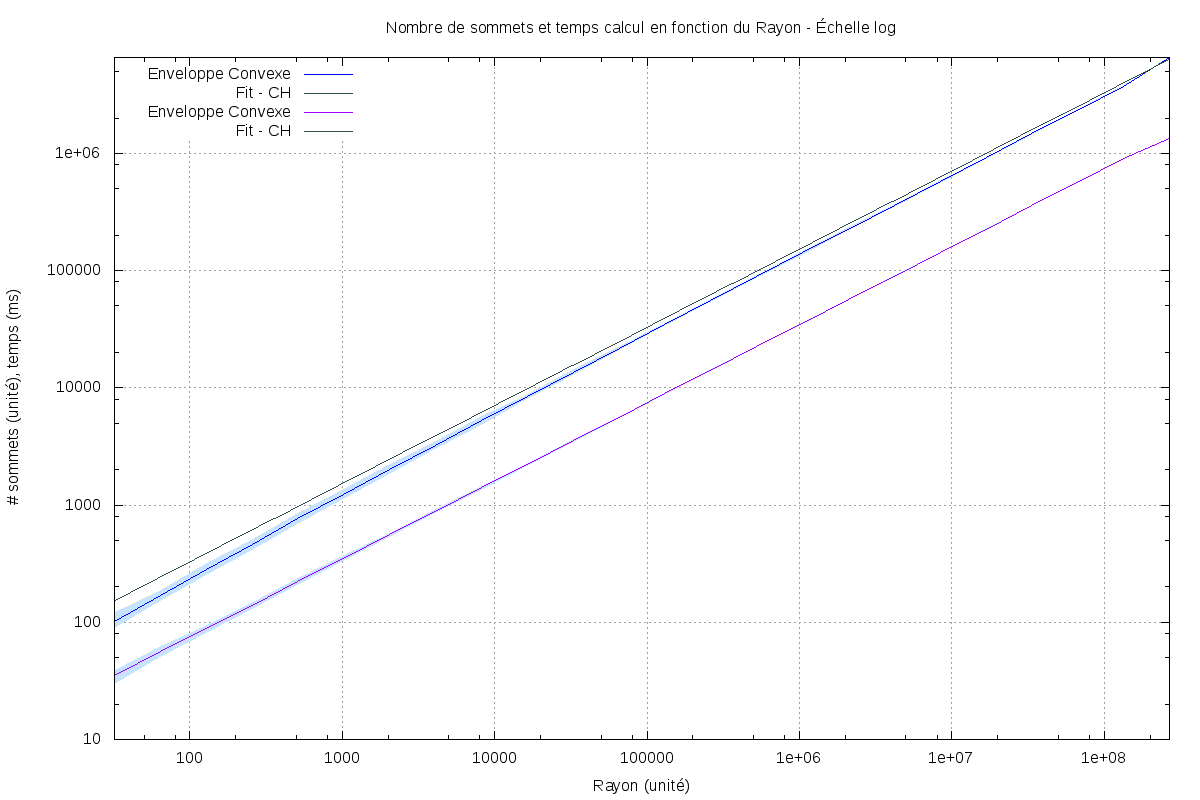
\includegraphics[width=\linewidth]{fig/4-exi/ch/exi-ch-sommet.png}
  \caption{Nombre de sommets de l'$\alpha$-shape en fonction de la taille des rayons. (Échelle log)}
\end{figure}


\begin{table}[H]
  \begin{tabular}{|p{0.09\linewidth}|p{0.13\linewidth}||p{0.23\linewidth}||p{0.23\linewidth}|p{0.23\linewidth}|}
    \hline
    \multicolumn{2}{|c||}{Rayon} & prédicat               & \multicolumn{2}{|c|}{$\alpha-shape$} \\  \hline 
    $R=2^k$  &                   & $-\alpha = R^{2}/1000$ & \multicolumn{2}{|c|}{Nombre de sommets} \\ \hline
    k        & R                 &                        & \# & $\# / R^{2/3}$ \\ 
    \hline
    5 & 32 & 1,024 & 179,02 & 17,761\\
    6 & 64 & 4,096 & 272,92 & 17,0575\\
    7 & 128 & 16,384 & 472,19 & 18,5913\\
    8 & 256 & 65,536 & 774,45 & 19,2088\\
    9 & 512 & 262,144 & 1,30E+03 & 20,3259\\
    10 & 1024 & 1,05E+03 & 2,14E+03 & 21,0878\\
    11 & 2048 & 4,19E+03 & 3,54E+03 & 21,9549\\
    12 & 4096 & 1,68E+04 & 5,68E+03 & 22,1878\\
    13 & 8192 & 6,71E+04 & 9,25E+03 & 22,7644\\
    14 & 16384 & 2,68E+05 & 1,49E+04 & 23,0413\\
    15 & 32768 & 1,07E+06 & 2,38E+04 & 23,2816\\
    16 & 65536 & 4,29E+06 & 3,84E+04 & 23,6175\\
    17 & 131072 & 1,72E+07 & 6,17E+04 & 23,9124\\
    18 & 262144 & 6,87E+07 & 9,89E+04 & 24,15\\
    19 & 524288 & 2,75E+08 & 1,59E+05 & 24,4137\\
    20 & 1048576 & 1,10E+09 & 2,54E+05 & 24,5914\\
    21 & 2097152 & 4,40E+09 & 4,06E+05 & 24,7603\\
    22 & 4194304 & 1,76E+10 & 6,49E+05 & 24,9402\\
    23 & 8388608 & 7,04E+10 & 1,04E+06 & 25,073\\
    24 & 16777216 & 2,81E+11 & 1,65E+06 & 25,2002\\
    25 & 33554432 & 1,13E+12 & 2,63E+06 & 25,3061\\
    26 &  &  &  & \\
    27 &  &  &  & \\
    28 &  &  &  & \\
    \hline
  \end{tabular} 
  \caption{Nombre de sommets de l'$\alpha$-shape}
\end{table}


%-----------------------------------------------------------------
\subsection{$\alpha$-shape, $\alpha \geq 0$}
%-----------------------------------------------------------------

%-----------------------------------------------------------------
\subsubsection{Construction de l'algorithme}

La méthode de calcul de l'$\alpha$-shape pour $\alpha > 0$ est fondamentalement différentes des méthodes de calculs présentées précédemment. La méthode n'est plus incrémentale mais de type ``Bottom-Up''. L'algorithme part du cas critique de l'enveloppe convexe. L'ensemble des sommets de l'$\alpha$-shape est un sous-ensemble des sommets de l'enveloppe convexe. 

L'algorithme commence également différement des autres déjà présentés. Le départ est en deux phases. Il faut d'une part récupérer un point de départ pertinent mais également l'ensemble des sommets de l'enveloppe convexe. Le point d'ordonnée minimale et d'abscisse maximale n'est plus néccéssairement dans l'$\alpha$-shape. Un mauvais point de départ engendrerait un calcul potentiellement faux. Pour être certain de notre départ, nous ne le calculons pas mais le choisissons par construction parmi l'un des trois sommets du triangle composant le cercle circonscrit. Ensuite, nous récupérons à partir de ce point l'ensemble des sommets de l'enveloppe convexe du disque discret. On note $\mathcal{S}$ cet ensemble.

\begin{figure}[H]
  \centering
  \includegraphics[width=0.5\linewidth]{fig/5-con/pas/con-pas-0.pdf}
  \caption{Le cercle circonscrit au triangle et l'enveloppe convexe de son disque.}
\end{figure}


Notons a,b et c trois sommets successifs appartenant à S. Supposant que a appartient à l'$\alpha$-shape, nous allons vérifier la présence de b et c dans l'$\alpha$-shape. Nous utilisons prédicat qui compare la taille du rayon \textbf{$R_T$} du cercle circonscrit au triangle : $T(a, b, c)$ à la taille du rayon de notre disque généralisé : \textbf{$R_{\alpha}$} $= 1/\alpha$. Il faut distinguer deux cas de figures.\\



On note $b = p_{k-2} + (q_k - 1) * p_{k-1}$ et $c = p_k = p_{k-2} + q_k * p_{k-1}$. Pour savoir si c est un sommet, on utilise un prédicat qui compare la taille du rayon \textbf{$R_T$} du cercle circonscrit au triangle : $T(a, b, c)$ à la taille du rayon de notre disque généralisé : \textbf{$R_{\alpha}$} $= 1/\alpha$. Il faut distinguer deux cas de figures.\\

\begin{figure}[H]
  \centering
  \includegraphics[width=0.6\linewidth]{fig/5-con/nas/con-nas-1.pdf}
  \caption{Calcul du Prédicat}
\end{figure}


Si $\alpha = \alpha_{1}$ alors \textbf{$R_{\alpha_{1}} < R_T$} et le point b appartient au notre disque généralisé de rayon $-1/R_{\alpha_{1}}$. Il est possible de rejoindre c par a à l'aide d'un arc de cercle dont le disque comprend l'ensemble des points de $\mathcal{D}$. b appartient à l'$\alpha$-hull, mais n'appartient pas à l'$\alpha$-shape. On continue la procedure pour étudier les sommets suivants. a reste inchangé, b devient c et c devient le sommet suivant de $\mathcal{S}$.

\begin{figure}[H]
  \centering
  \includegraphics[width=0.4\linewidth]{fig/5-con/pas/con-pas-1.pdf}
  \includegraphics[width=0.4\linewidth]{fig/5-con/pas/con-pas-2.pdf}
  \caption{Calcul du Prédicat}
\end{figure}

Si $\alpha = \alpha_{2}$ alors \textbf{$R_{\alpha_{2}} > R_T$} et le point b n'appartient pas à notre disque généralisé de rayon $1/R_{\alpha_{1}}$. L'$\alpha$-hull ne peut rejoindre c par a sans au moins passé par b. \textbf{b appartient à l'$\alpha$-shape}. Il faut poursuivre la procédure afin de réaliser un tour complet. b devient a, c devient b et c devient le sommet suivant de $\mathcal{S}$.\\

\begin{figure}[H]
  \centering
  \includegraphics[width=0.4\linewidth]{fig/5-con/pas/con-pas-3.pdf}
  \includegraphics[width=0.4\linewidth]{fig/5-con/pas/con-pas-4.pdf}
  \caption{Calcul du Prédicat}
\end{figure}

%-----------------------------------------------------------------
\subsubsection{Résultats}

\begin{figure}[H]
  \centering
  %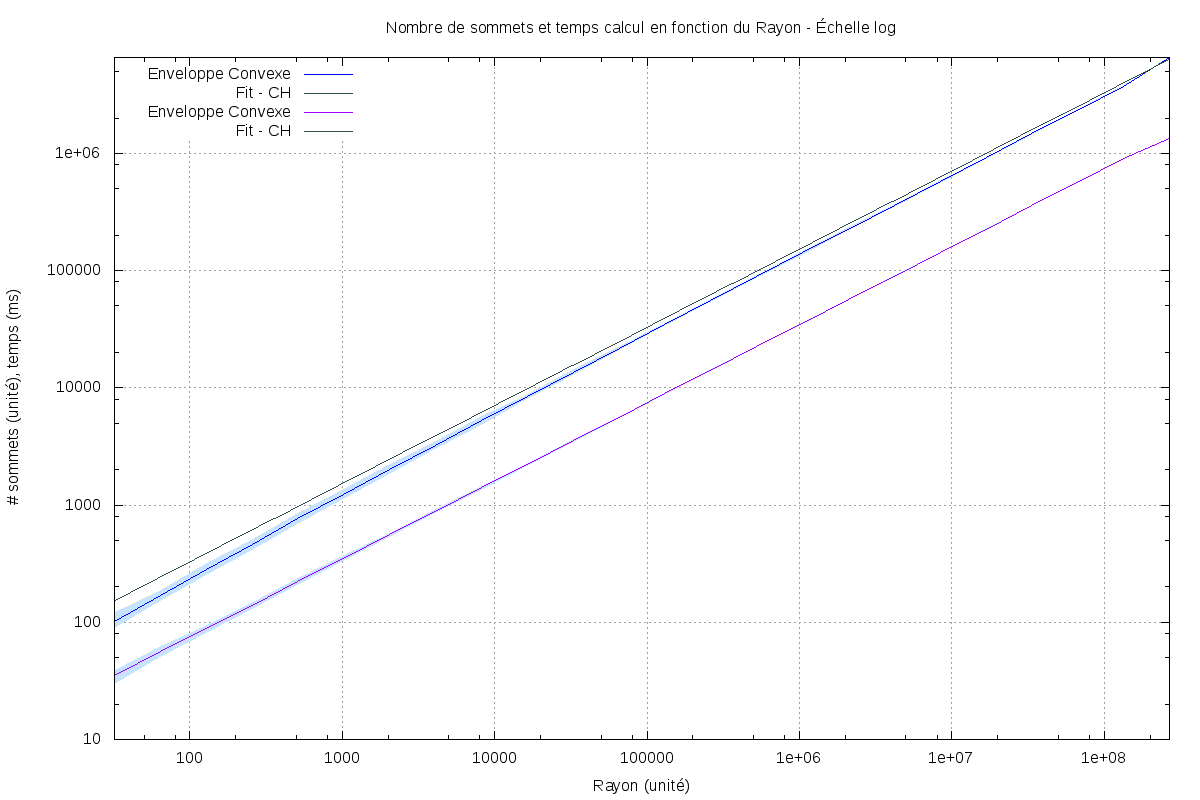
\includegraphics[width=\linewidth]{fig/4-exi/ch/exi-ch-sommet.png}
  \caption{Nombre de sommets de l'$\alpha$-shape en fonction de la taille des rayons. (Échelle log)}
\end{figure}


\begin{table}[H]
  \begin{tabular}{|p{0.09\linewidth}|p{0.13\linewidth}||p{0.23\linewidth}||p{0.23\linewidth}|p{0.23\linewidth}|}
    \hline
    \multicolumn{2}{|c||}{Rayon} & prédicat               & \multicolumn{2}{|c|}{$\alpha-shape$} \\  \hline 
    $R=2^k$  &                   & $-alpha = k*R^{2}$ & \multicolumn{2}{|c|}{Nombre de sommets} \\ \hline
    k        & R                 &                        & \# & $\# / R^{2/3}$ \\ 
    \hline
    
    \hline
  \end{tabular} 
  \caption{Nombre de sommets de l'$\alpha$-shape}
\end{table}


%------------------------------------------------
\section{Développement Informatiques}
%------------------------------------------------

%-----------------------------------------------------------------
\subsection{Programmation}
%-----------------------------------------------------------------

%-----------------------------------------------------------------
\subsubsection{C++}

Le C++ est un langage de programmation né dans les années 1980 dans l'optique d'agrémenter le langage C de nouvelles fonctionnalités. Il fut d'abord nommée par son créateur Bjarne Stroustrup : C with Classes. L’appellation c++, rappelant l'opération d'incrémentation fut adopté peu de temps plus tard à partir de 1983 suite à l'ajout de nouvelles fonctionnalités. (Source \cite{Wiki-cpp})

Aujourd'hui encore, de nombreuses fonctionnalités viennent agrémenter le langage C++ au fil des spécifications. Il est désormais possible de l'utiliser en s'appuyant sur de multiples paradigmes comme la programmation procédurale, la programmation orientée objet et la programmation générique.

Le paradigme choisit dans ce stage est celui de la programmation générique. \cite{troussil-cpp}

%-----------------------------------------------------------------
\subsubsection{Programmation générique}


Le paradigme de la programmation générique s'appuie sur des relations concepts-modèles entre les types de données.  

Pour appartenir à un même concept, les types doivent posséder un même interface. 

\begin{Definition}{Concept}\\
\label{def:cpp-con}
    Un concept définit une interface en terme de données, méthodes et types internes. Il rassemble des contraintes syntaxiques (les noms sont fixes) et sémantiques (les comportements doivent être équivalents). 
\end{Definition}

\begin{Definition}{Modèle}\\
  Un modèle est un type qui satisfait les contraintes d'un concept.
\label{def:cpp-mod}

\end{Definition}

On parle alors de polymorphisme statique dans le sens où un algorithme, une fonction peut s'exécuter avec des types différents.

%-----------------------------------------------------------------
\subsubsection{Exemple concret}

% Points

L'espace de travail $\mathbb{Z}^{2}$ est une grille régulière représentant des points à coordonnées entières. Ce sont les principaux objets que nous allons manipuler. L'un des enjeux de la géométrie discrète est de baser ses calculs principalement sur l'usage d'entiers afin d'éviter tous les problèmes apportés par les incertitudes de précision dû aux flottants. Comme le C++ est un langage fortement typé, la représentation des entiers diffère selon la taille maximale autorisée souhaitée. On parle alors de concept d'``Entier''. Plusieurs modèles de base sont présents : int, long. Nous utiliserons également un modèle BigInteger intégré par l'intermédiaire des librairie DGtal et GMP qui permet de manipuler de très grands entiers.

Nous avons aussi un concept de ``Point''. Dans un premier temps, nous avons implémenté une classe PointVector2d, comme un modèle de ``Point''. Dans un second temps, nous avons utilisé le modèle PointVector de la librairie DGtal.  

\begin{figure}[H]
  \centering
  \includegraphics[trim = 2cm 14cm 2cm 2cm, clip, width=0.5\linewidth, ]{fig/6-info/dia-conv.pdf}
  \caption{Modèles et concepts utilisés.}
\end{figure}

%% Notre classe point possède deux variables internes myX et myY de type Entier. Elle est muni de diverses opérations.

%% TRI pas utile!
%% ce que je demandais, ce sont les opérations associés à un concept pas à une classe. 
%% \begin{table}[H]
%%   \begin{tabular}{|p{0.2\linewidth}|p{0.7\linewidth}|}
%%     \hline
%%      Opérations & Fonctionalités\\ 
%%     \hline
%%     +, -               & Addition et Soutraction\\
%%     =                  & Affectation par un autre point\\
%%     +=, -=             & Addition, soustraction et affectation\\
%%     ==, !=             & Comparaison\\
%%     $[i], i = 1 \text{ ou } 2$     & Accès aux coordonnées\\
%%     (,)                & Affectation par les coordonnées\\
%%     normL1(), normL2() & Diverses normes\\
%%     std::cout          & Sortie standart\\
%%     \hline
%%   \end{tabular} 
%%   \caption{Nombre de sommets de l'$\alpha$-shape}
%% \end{table}

Pour mettre en oeuvre nos méthodes de calcul sur des objets dans $\mathbb{Z}^{2}$ , nous avons implémenté un concept de ``FormeIntersectable'', 
représentant un objet géométrique pour lequel on est capable de calculer son intersection avec un rayon. Les modèles de ``FormeIntersectable''
doivent posséder au moins trois méthodes: 

\begin{itemize}
  \item un opérateur parenthèse pour le prédicat de position : est point est-il à l'intérieur ou à l'extérieur de la forme ?
  \item une méthode dray: le rayon émanent d'un point donné, dans une direction donnée intersecte-t-il cette forme et si oui, quelle est le point le plus proche et du même côté ?
  \item une méthode getConvexHullVertex pour obtenir le point de départ, situé à l'intérieur avec l'ordonnée minimale et l'abscisse maximale. 
\end{itemize}

Pour le moment, trois modèles ont été implémentés : RayIntersectableStraightLine (pour un segment de droite discrète), ExactRayIntersectableCircle (pour un disque discret implémentées avec des calculs sur des entiers), InexactRayIntersectableCircle (pour un disque discret implémentées avec des calculs sur des entiers et des flottants).

% graph contexte

%\newpage
%-----------------------------------------------------------------
\subsubsection{Dans la pratique}

Le code suivant permet de stocker les sommets de l'enveloppe convexe
d'un disque discret dans un STL vector. 

\begin{verbatim}
  ... // Lire a, b, c, d

  // On définit un disque de paramètres a, b, c, d
  // tels que ax + by + c(x^2 + y^2) + d <= 0
  Disk aDisk( a, b, c, d );	 
  
  // Déclaration de l'enveloppe convexe de notre disque.
  OutputSensitiveConvexHull<Disk> algo(aDisk);
  
  // Variable stockant les sommets succéssifs.
  std::vector<Point> convexHullVertices
  
  // Récupération des sommets par un itérateur 
  algo.all( std::back_inserter( convexHullVertices ) );  
\end{verbatim}

Auparavant, on a le choix d'utiliser différents modèles de disques. 
Soit un modèle où les calculs sont possiblement inexacts (mais plus rapides): 
\begin{verbatim}
  typedef InexactRayIntersectableCircle<int> Disk;
\end{verbatim}
Soit un modèle où les calculs sont exacts (mais plus lents):
\begin{verbatim}
  typedef ExactRayIntersectableCircle<DGtal::BigInteger> Disk;
\end{verbatim}

La programmation générique nous a permis d'implémenter qu'une seule fois la classe OutputSensitiveConvexHull et sa méthode all qui récupère les sommets de l'enveloppe convexe. Nous avons pu ainsi utiliser nos méthodes sur différents modèles en toute transparence. 
%Néanmoins la réalisation d'un projet comportant du développement informatique impose certaines contraintes au niveau du rendu. 

%-----------------------------------------------------------------
\subsection{Génie logiciel}
%-----------------------------------------------------------------

%-----------------------------------------------------------------
\subsubsection{Tests}

Le but de tout algorithme est de répondre juste à la question qui lui est posée. L'une des difficultés rencontrés dans ce stage reste la faible présence d'outils susceptibles de nous répondre à notre question par d'autre chemin. Pour vérifier nos calculs, nous avons implémenté des méthodes de tests s'appuyant sur le suivi de bord pour les méthodes recherchant des bords. En codant les tests unitaires avant nos méthodes de calcul, nous avons mis en place une logique de développement par les tests. 
%% utilisant le principe : Stop The line. \cite{stoptheline}
%%TRI: pas très pertinent

Dans le cadre d'un développement informatique, cela consiste à essayer de provoquer l'ensemble des cas critiques et de chercher à les passer. Le but étant de pouvoir utiliser le code en production en minimisant le risque de trouver un résultat incorrect.\\

Les tests unitaires ont été générés aléatoirement sur un grand nombre de cas et se sont concentré sur certains cas particuliers critiques. Ses tests ont été automatisés avec l'utilisation de make et cmake. L'appel à la commande make test permettant de lancer tous les tests et d'ainsi vérifier l'intégration et la non-régression lors de l'ajout de nouvelles méthodes. 


%-----------------------------------------------------------------
\subsubsection{Espace de collaboration}

Le projet crée à l'occasion de ce stage a été de développer des méthodes en s'appuyant sur un projet de plus grande envergure à travers l'utilisation de la librairie DGtal : \cite{DGtal}. Afin d'être compatible, il faut accepter de suivre un certain formalisme pour homogénéiser l'ensemble. Il faut suivre les conventions établies au niveau du nommage des variables, de la mise en place des commentaires et de la documentation. Une autre forme de formalisme à suivre se retrouve également à travers l'écriture directe du programme et de la gestion des longues lignes de codes et tout simplement des tabulations/espaces afin de pouvoir tirer au mieux profit de la puissance des gestionnaires de version, de git dans notre cas.\\

La collaboration avec mon encadrant s'est grandement appuyée sur l'utilisation quotidienne du logiciel git et de l’hébergement de notre projet sur la plateforme github : \cite{github-tristan} et \cite{github-thomas} permettant de garder facilement une trace des travaux et modifications effectués. Environ 270 commits sont venus répondre à une soixantaine de problèmes soulevés.\\

Un projet informatique n'a de sens et d'utilité que s'il est complet. Il est important dans un souci de pérennité de proposer un travail fini afin que celui-ci puisse être compris et utilisé ultérieurement. Cela a été l’occasion de retravailler le projet dans son ensemble avec du recul pour par exemple nommer correctement et avec des noms cohérents l'ensemble des classes.

%-----------------------------------------------------------------
\subsubsection{Structure du dépôt}


Le dépôt est structuré en plusieurs fichiers et dossiers.

\begin{itemize}
  \item doc contient l'ensemble des présentations, rapports et algorithmes créés à l'occasion de ce stage. Les formats texte et xml ont été privégiés afin de pouvoir utiliser au mieux git.
  \item inc (10 fichiers ) contient les modèles et les méthodes développés en c++. 
  \item stests (8 fichiers ) contient l'ensemble des tests développés afin de vérifier nos modèles et méthodes.
  \item stools (3 fichiers ) contient deux outils qui récupèrent les résultats de nos méthodes.
  \item tools (2 fichiers ) contient des scripts GNUPlot pour tracer les graphiques à partir des résultats.
\end{itemize}

Afin d'utiliser au mieux notre projet il faut maintenant installer la librairie DGtal \cite{DGtal}. Les prérequis sont cmake, boost et GMP (Gnu Multiprecision Arithmetic Library). 

Afin de construire et utiliser les différents programmes créés il faut suivre la procédure suivante :

\begin{itemize}
  \item Créer un répertoire de construction : mkdir build; cd build
  \item Genererer les makefiles : cmake ..
  \item Compiler, créer les executables : make
  \item Éxecuter tous les tests : make test
  \item Éxecuter un test particulier : ./stests/test*
  \item Utiliser un outil : ./stools/tool*
\end{itemize}



%------------------------------------------------
\section{Conclusion}
%------------------------------------------------

%-----------------------------------------------------------------
\subsection{Poursuite du projet}
%-----------------------------------------------------------------

Le projet scientifique commencé par l'intermédiaire de ce stage peut être étendu sur bien des points. 

Sur le plan du développement informatique, il reste possible d'ajouter de nombreuses fonctionnalités. L'etude d'autres formes géométriques comme l'ellipse, l'union de deux droites discrètes semble être des ajouts intéressants. L'implémentation différentes des algorithmes déjà présents permettrait de mieux cerner les optimisations possibles et d'ainsi mieux cerner les contraintes et choix techniques a éffectuer ultérieurement. En s'intéressant au calcul des $\alpha$-shapes par arête de l'enveloppe convexe permettrait de tirer profit d'une possible parallélisation où bien d'une table de hâchage afin de conserver les points ajoutés pour les arêtes. Inversement, adopter une approche commençant du polygone minimal afin de remonter vers l'$\alpha$-shape quand $\alpha > 0$ serait une méthode avec une compléxité qui deviendrait intéressant à partir d'un certain rapport Rayon du disque / $\alpha$.

Un projet plus ambitieux et plus long serait de chercher à généraliser la méthode à la dimension 3 même s'il faudrait repartir d'une nouvelle base avec des points dans $\mathbb{Z}^{3}$. 

Un autre intérêt scientifique serait d'approfondir les résultats obtenus en réalisant une étude asymptotique du nombre de sommet d'une $\alpha$-shape en fonction de $\alpha$ et de R, le rayon du disque.

Enfin, le but de tout algorithme étant d'être utilisé, il serait intéressant une fois le projet achevé de chercher à l'intégrer à la librairie DGtal afin de pouvoir utiliser les $\alpha$-shapes dans un cadre de reconnaissance de forme et d'échantillonage \cite{BernardiniB97}.


%-----------------------------------------------------------------
\subsection{Compétences acquises}
%-----------------------------------------------------------------


Apprentisage en Informatiques
-C++, découverte de la programmation générique à base de template.
-Utilisation de make, cmake.
-Utilisation quotidienne de Git.

Découverte de la géométrie discrète.

%-----------------------------------------------------------------
\subsection{Ouverture personnelle}
%-----------------------------------------------------------------






%\part{Développement informatiques}
%%%%%%%%%%%%%%%%%%%%%% chapter.tex %%%%%%%%%%%%%%%%%%%%%%%%%%%%%%%%%
%
% sample chapter
%
% Use this file as a template for your own input.
%
%%%%%%%%%%%%%%%%%%%%%%%% Springer-Verlag %%%%%%%%%%%%%%%%%%%%%%%%%%


\chapter{Environnement de travail}
\label{pt2-ch1-et} % Always give a unique label
% use \chaptermark{}
% to alter or adjust the chapter heading in the running head

\section{Environnement matériel et logiciel}
\label{pt2-ch1-sec:1}

\section{Paradigme de Programmation}
\label{pt2-ch1-sec:2}

\section{Espace de collaboration}
\label{pt2-ch1-sec:3}

\chapter{Structure du code}
\label{pt2-ch2-sd} % Always give a unique label

\section{Principaux concepts}
\label{pt2-ch2-sec:1}

\section{Installation et utilisation}
\label{pt2-ch2-sec:2}

\subsection{Librairies et licence}
\label{pt2-ch2-sec:2:1}

Le code source de ce présent projet est disponible sous les conditions de la licence GPLv3 \cite{GPLv3}. Néanmoins, il convient de remarquer que deux librairies sont utilisées directement : Boost (licence Boost  - \cite{boost-licence})) et DGtal (Licence GPLv3 - \cite{GPLv3}).

\subsubsection{Boost}

Boost \cite{boost} est une grosse librairie C++. \\
On remarque qu'elle est également utilisé par la libraire DGtal.\\

Son utilisation directe dans le cadre de ce projet est relativement parcimonieuse. En effet, son utilisation a été limité à \bsc{Program Options} pour la création d'une interface légère à base de paramètres à ajouter pour l’exécution des programmes commandant les sorties.


\subsubsection{DGtal}

DGtal \cite{DGtal} est une librairie developpé en partie en interne par des membres de l'équipe M2Disco en plus d'autres partenaires. Son objectif principal est de proposer des outils permettant de traiter de géométrie discrète. \\

Son utlisation est intervenu sur plusieurs plans. \\

(?? Utilisation de liste pour alléger un peu la partie ??)

L'avantage indéniable de faire des calculs avec seulement des entiers est de calculer de manière exacte. Néanmoins, une contrainte peut "vite" apparaitre en augmentant la taille des rayons. En effet le type int peut alors être débordé en trouvant un entier plus grand que le plus grand entier alors compréhensible par notre système. L'utilisation de la librairie DGtal a alors permis par l'intermédiaire de gmp d’utiliser de très grands entiers.\\

DGtal a également été utilisé dans le postprocessing pour tirer partie du tableau permettant d'obtenir des traces de nos enveloppes de cercles.

\subsection{Installation}
\label{pt2-ch2-sec:2:2}

\subsection{Utilisation}
\label{pt2-ch2-sec:2:3}






%\part{Conclusion}
%%%%%%%%%%%%%%%%%%%%%% chapter.tex %%%%%%%%%%%%%%%%%%%%%%%%%%%%%%%%%
%
% sample chapter
%
% Use this file as a template for your own input.
%
%%%%%%%%%%%%%%%%%%%%%%%% Springer-Verlag %%%%%%%%%%%%%%%%%%%%%%%%%%

\chapter{Conclusion}
\label{pt5-ch1-con} % Always give a unique label
% use \chaptermark{}
% to alter or adjust the chapter heading in the running head

% En premier lieu il faut faire une transition qui permettra de passer en douceur du développement à la conclusion ; il convient ensuite de passer à un résumé du développement, et enfin de faire une ouverture. La conclusion va du particulier vers le général, c’est-à-dire qu’elle suit le processus inverse de celui adopté dans l’introduction. 

%%%%%%%%%%%%%%%%%%%%%%%%%%%%%%%%%%%%%%%%%%%%%%%%%%%%%%%%%%%%%%%%%%%

\section{Développement}
\label{pt5-ch1-1}

\subsection{Transition}
\label{pt5-ch1-sec:1.1}

\subsection{Objectif}
\label{pt5-ch1-sec:1.2}

\section{Ouverture}
\label{pt5-ch1-sec:2}



%%%%%%%%%%%%%%%%%%%%%%%%%%%%%%%%%%%%%%%%%%%%%%%%%%%%%%%%%%%%%%%%%%%%%%

\end{document}





